\documentclass[8pt]{minimal}
\usepackage{amsmath}
\usepackage{amssymb}
\usepackage{esdiff}
% \usepackage{fullpage}
\usepackage{graphfig}
\usepackage{graphicx}
\usepackage{siunitx}
\usepackage{wrapfig}

\newcommand{\e}[1]{e^{#1}}
\newcommand{\ei}[1]{e^{i\left(#1\right)}}
\newcommand{\E}[1]{\times 10^{#1}}

\begin{document}
    \setlength{\parindent}{0pt}
    % \setlength{\voffset}{-50pt}
    \setlength{\columnsep}{0.5cm}
    % \setlength{\textheight}{length}
    \twocolumn
    PHYS 4D Lab Exam 2 Reference Sheet (with \LaTeX)

    \underline{Write Units}
    
    \underline{Fourier Analysis}\\
        Frequency domain shows spikes and amplitudes at discrete frequencies; $c = f\lambda$\\
        Square wave: Only odd numbered frequency spikes.
        \begin{equation*}
            g(t) = \sum_{n=1}^{\infty} \frac{4V_0}{n\pi}\sin(2\pi f_n t) \text{ for odd $n$}
        \end{equation*}
        Triangle wave: Similar to square wave; $f_n = nf_1$
        \begin{equation*}
            g(t) = \sum_{n = 1}^{\infty} (-1)^{\frac{n-1}{2}}\frac{8V_0}{n^2\pi^2}\sin(2\pi f_n t) \text{ for odd $n$}
        \end{equation*}

    \underline{Wave Packets}
        Localized particle uses localized wave; uses $\lambda = \frac{h}{p}$.
        Truly localized uses $\lim_{x \to 0^+} (x)$

        Shorter wavepackets $\to$ smaller frequencies

    \underline{LASER Sidelight}
        Light Amplification by Stimulated Emission of Radiation; 
        Light comes from Ne;
        He collide w/ Ne \& shift energy up;
        Only emits one color
        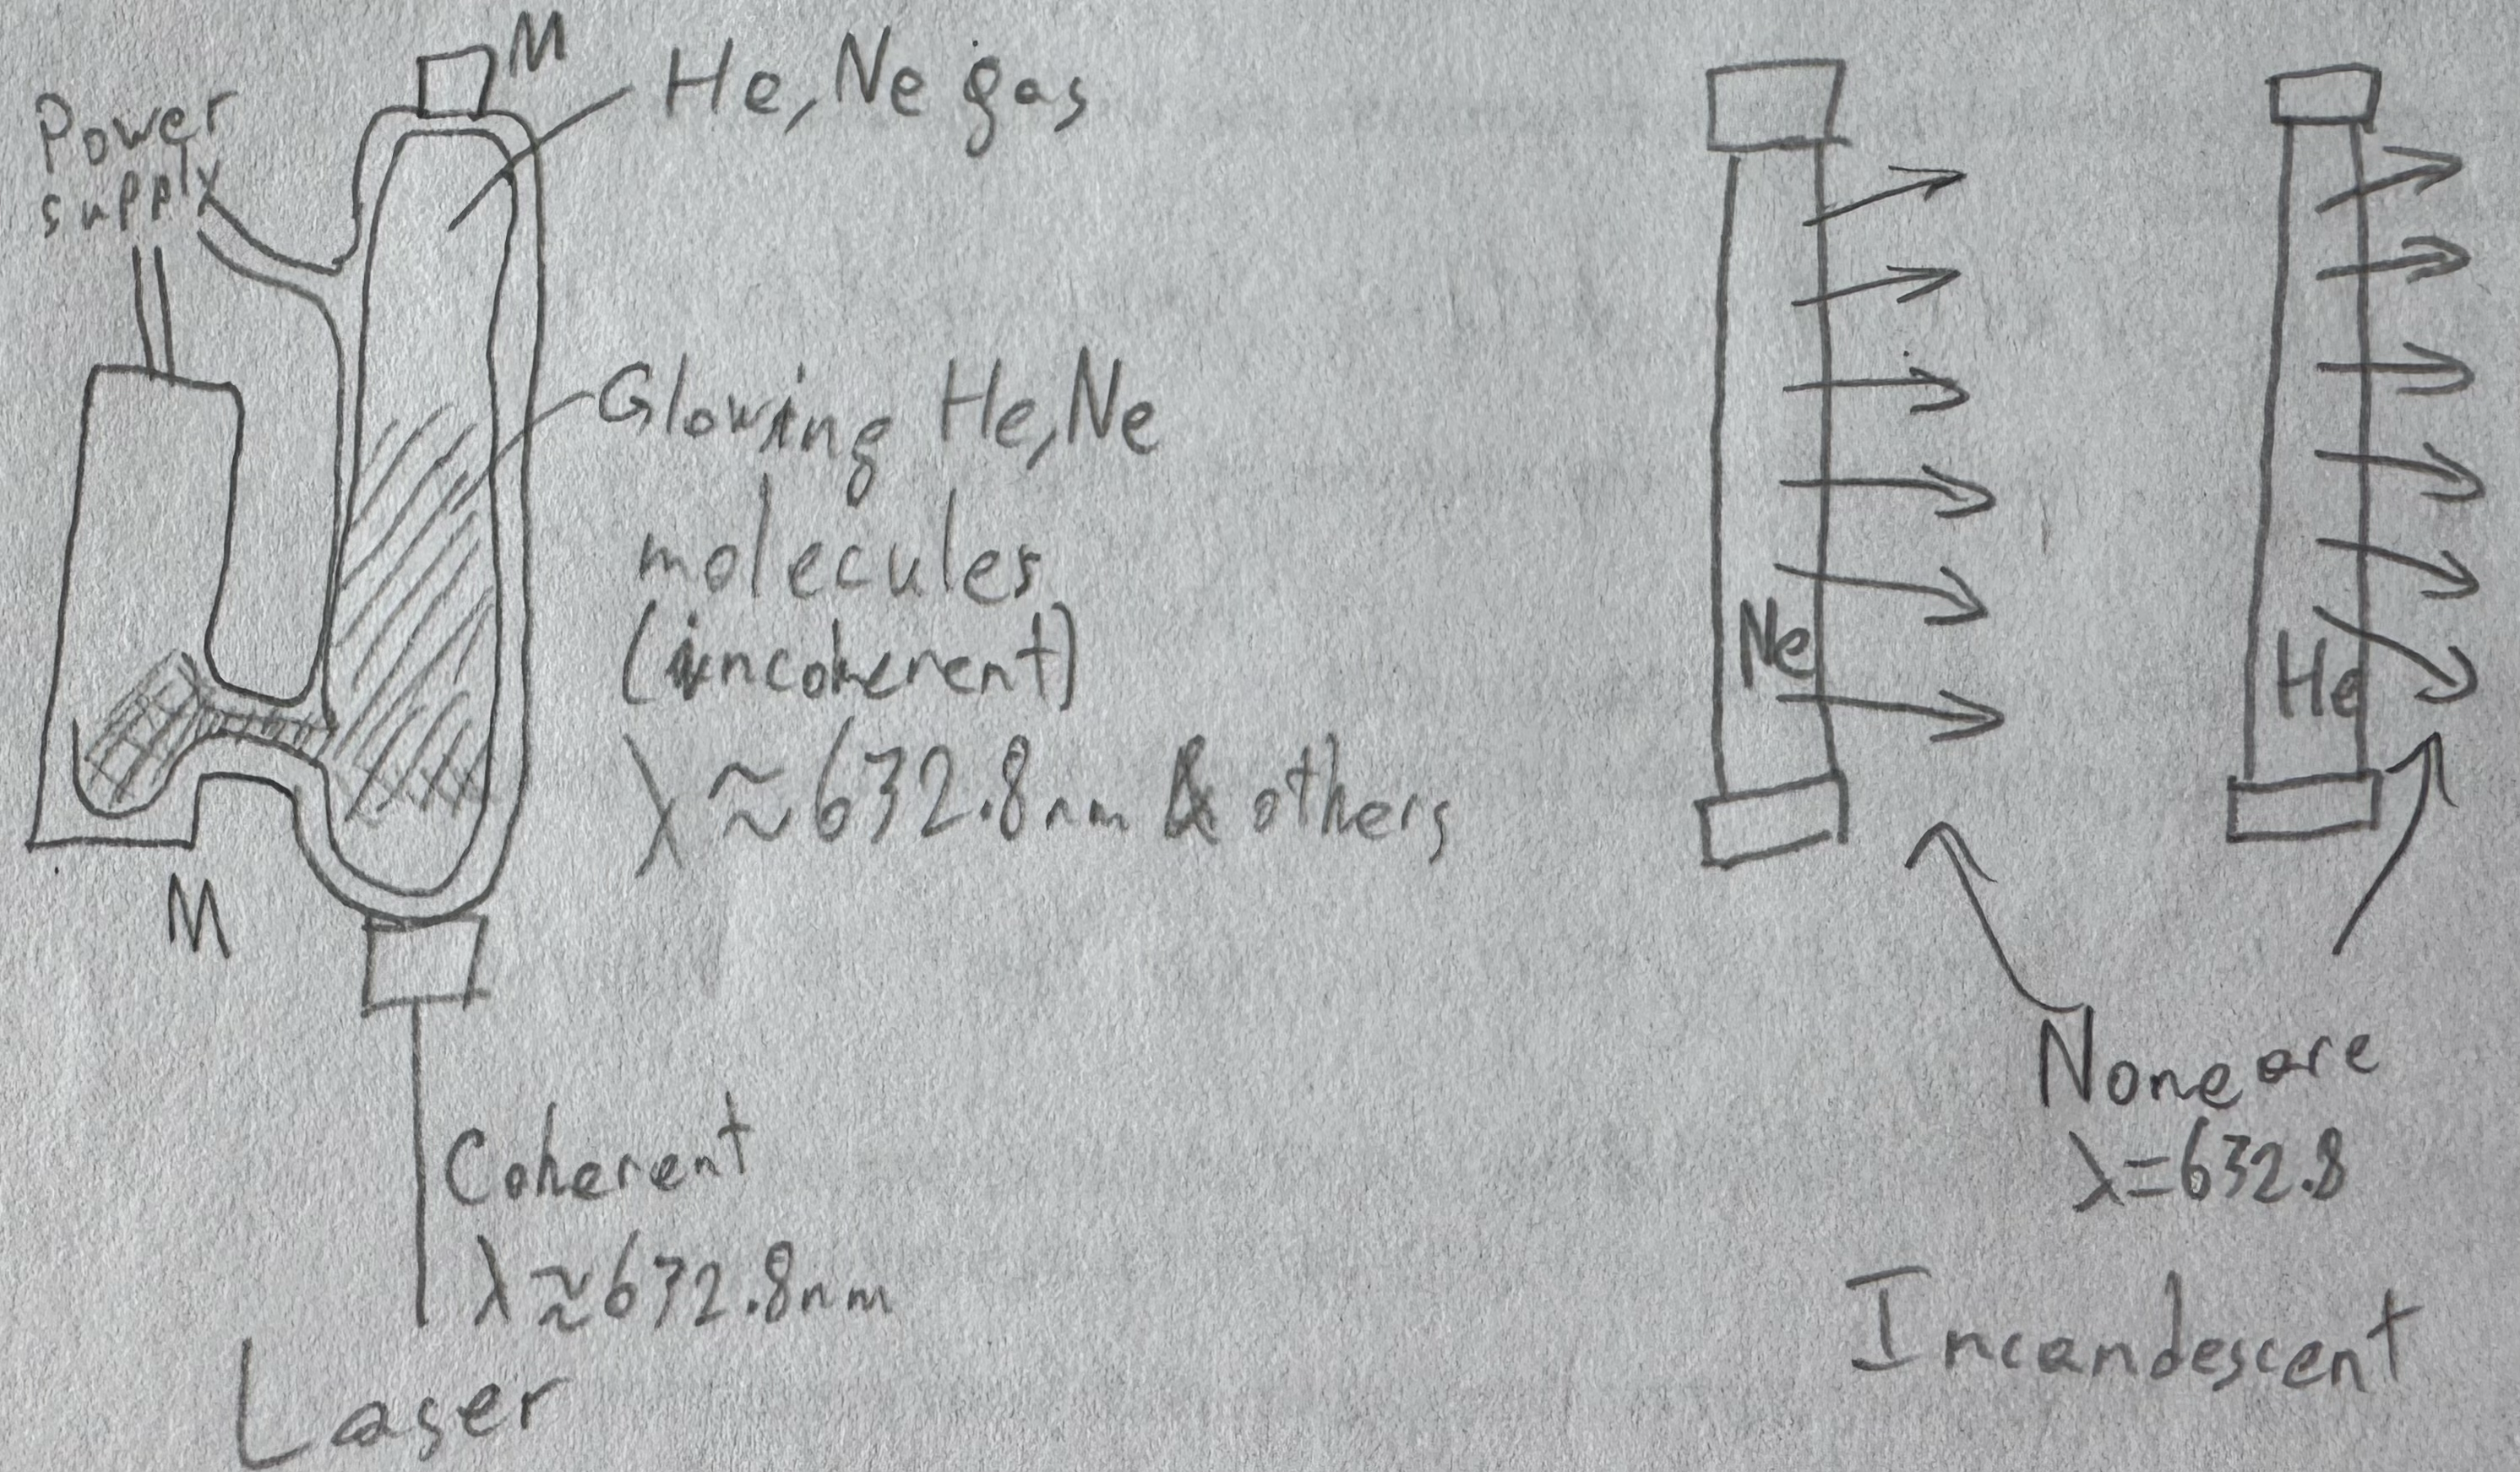
\includegraphics[width=0.25\textwidth]{Images/IMG_7626.png}
        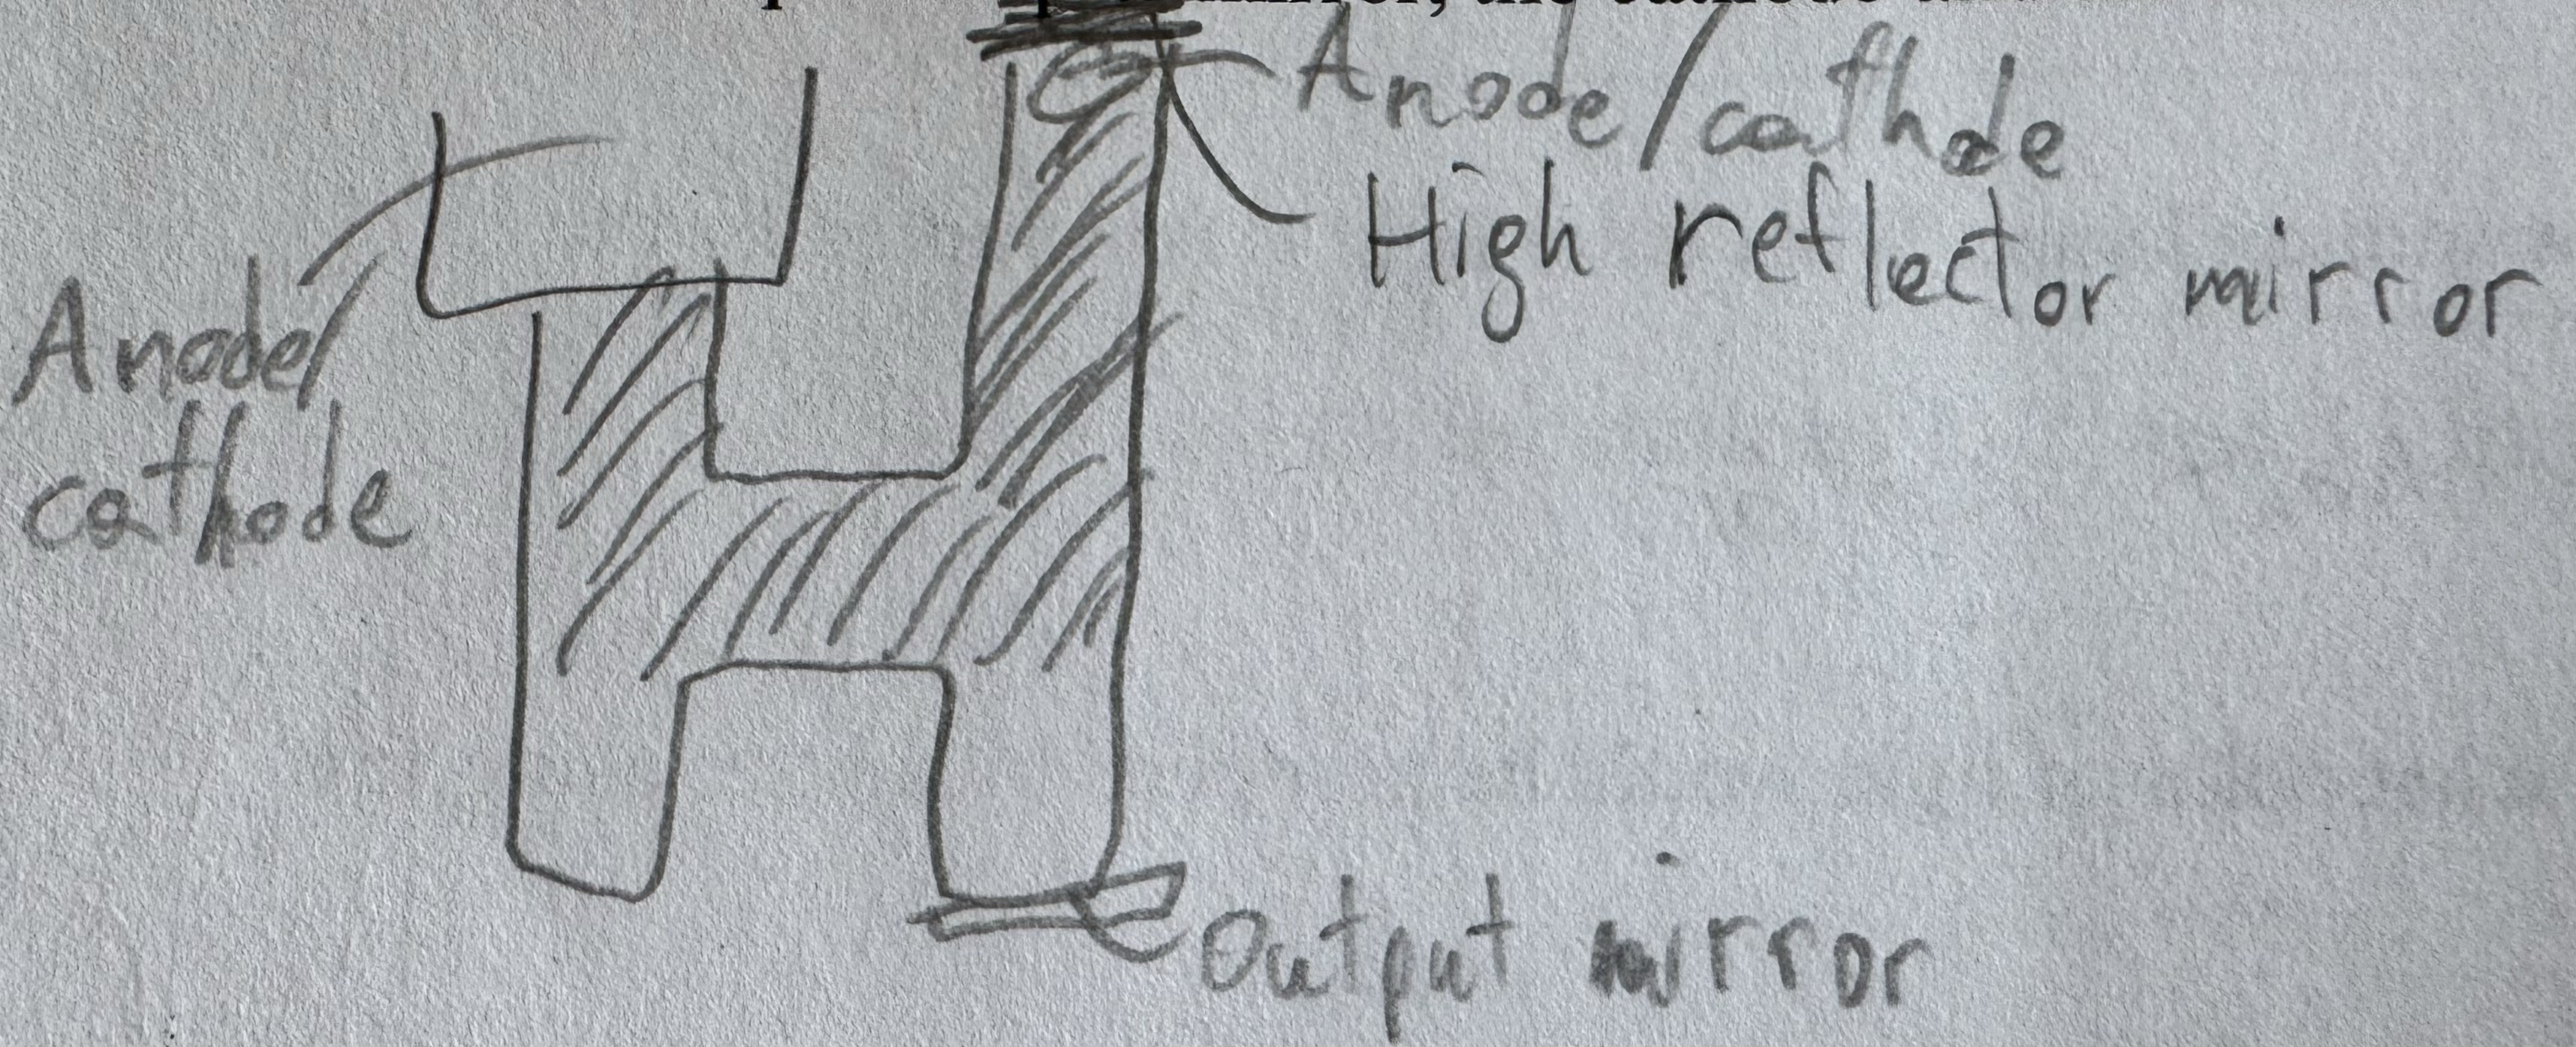
\includegraphics[width=0.23\textwidth]{Images/IMG_7627.png}
        Laser mirrors block one color but show the rest

    \underline{Longitudinal Modes; Zeeman Effect}
        Light in standing waves of tube width lare amplified ($\lambda_n = \frac{2L}{n}$);
        Doppler shift happens, wind up with beats

        \begin{wrapfigure}{r}{0.1\textwidth}
            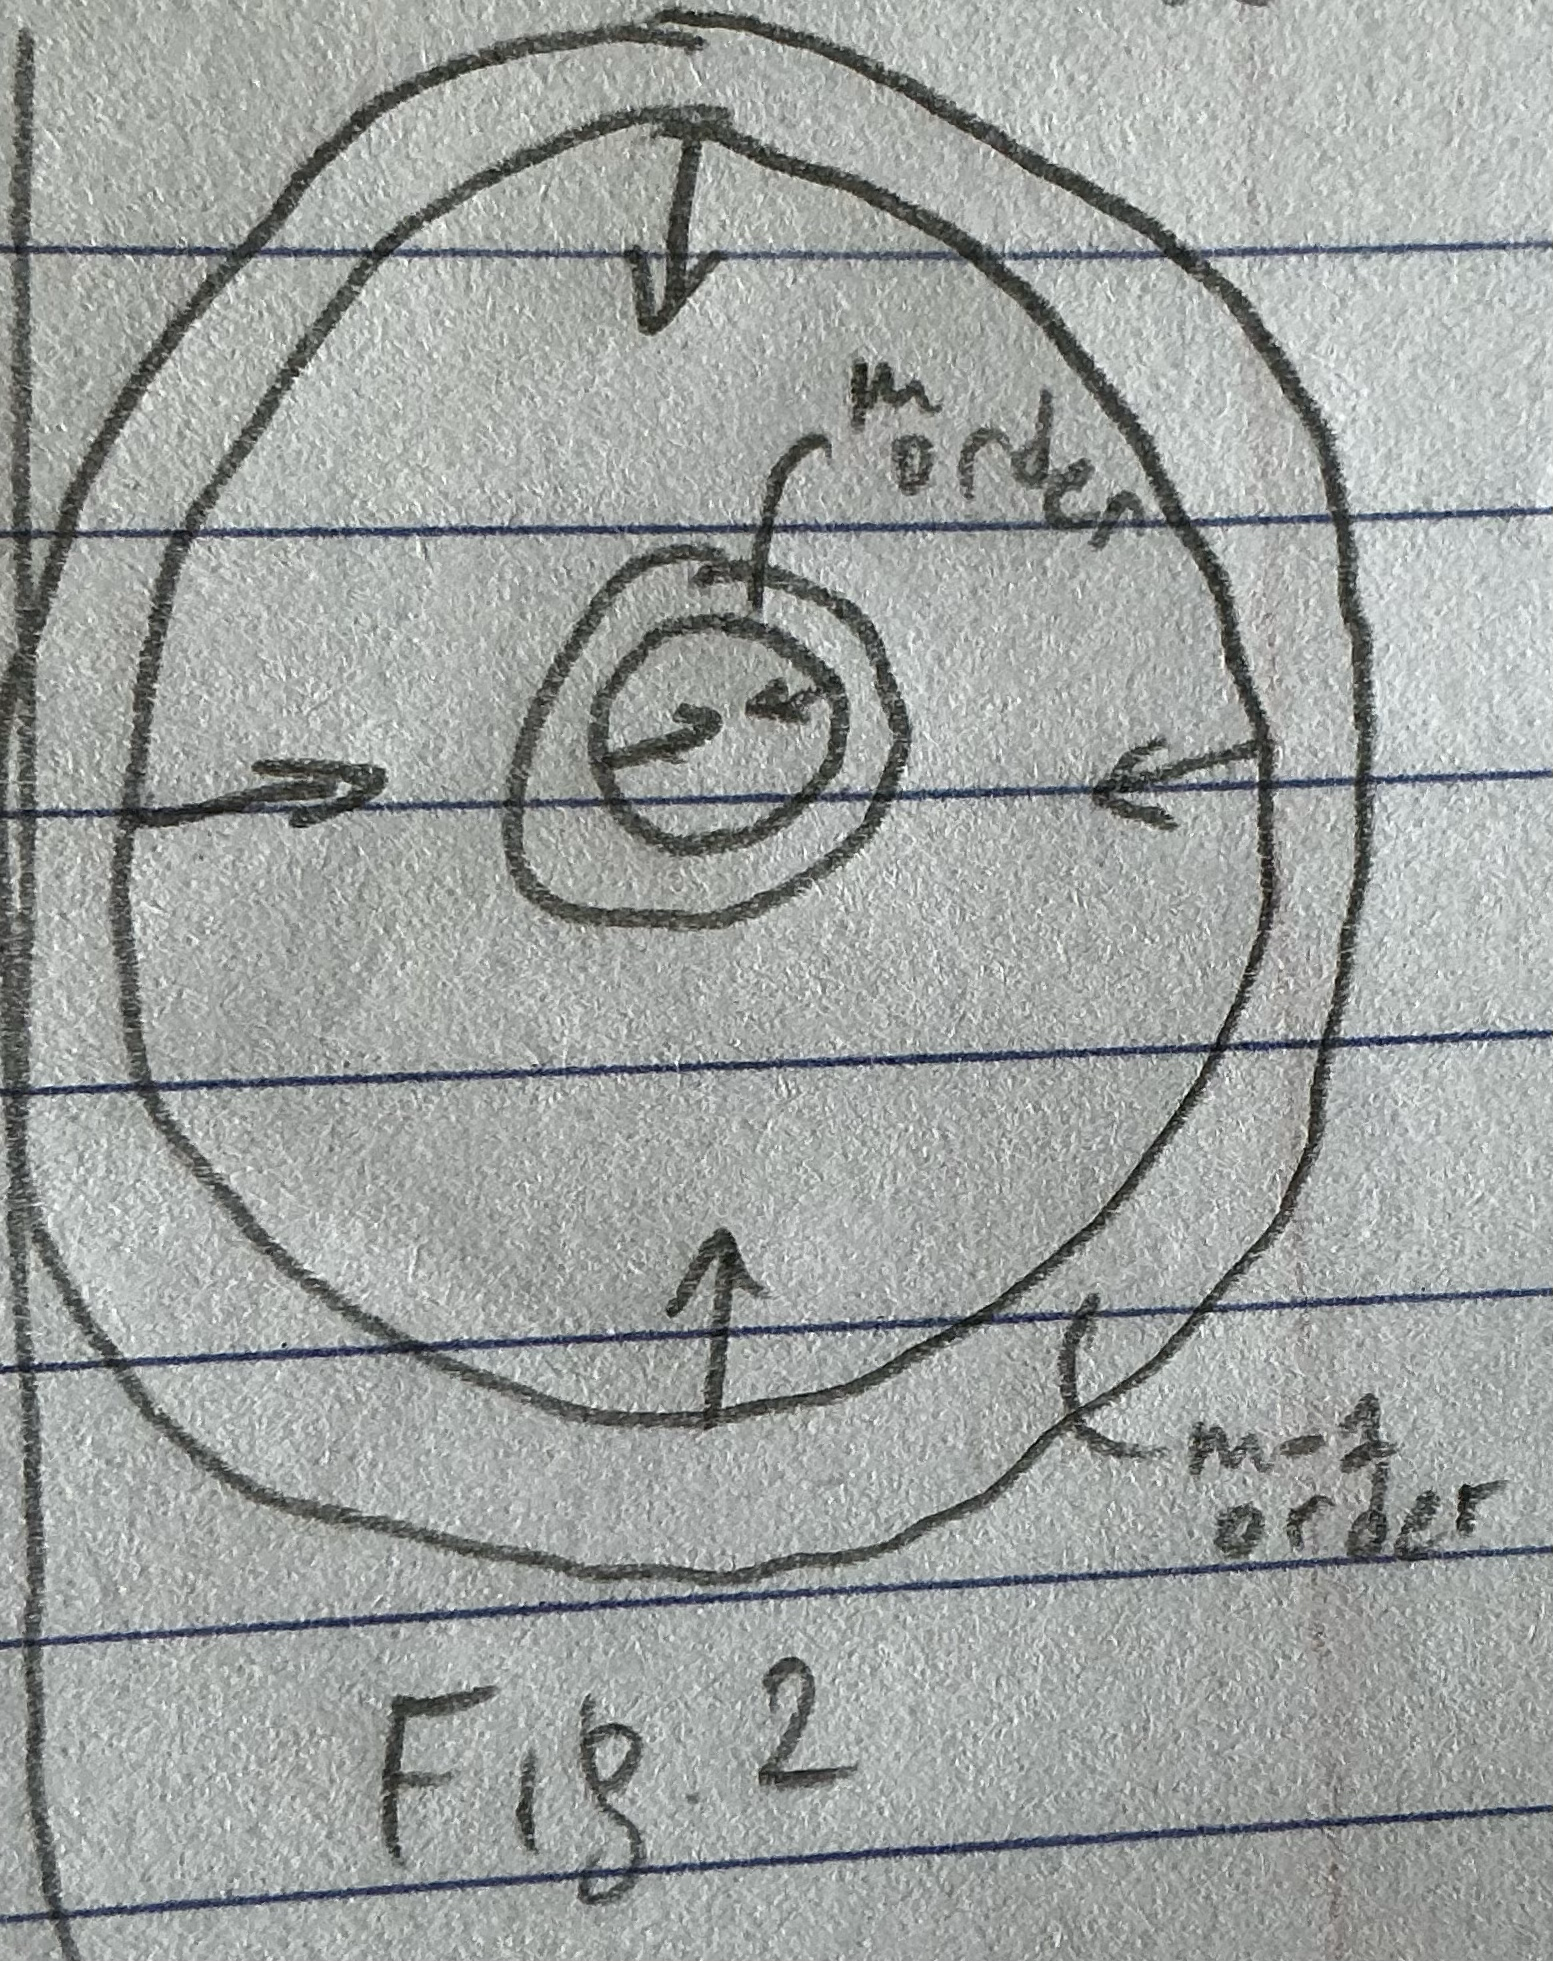
\includegraphics[width=0.1\textwidth]{Images/IMG_0227.png}
        \end{wrapfigure}
        \begin{gather*}
            \Delta m = \frac{D_m'^2 - D_m^2}{D_{m-1}^2 - D_m^2};
            \Delta f_{fsr} = \frac{c}{2d\mu_d}\\
            \mu_d = n - \lambda\diff{n}{\lambda};
            \Delta f = \Delta m \Delta f_{fsr}
        \end{gather*}
        As laser heats, more polarized

        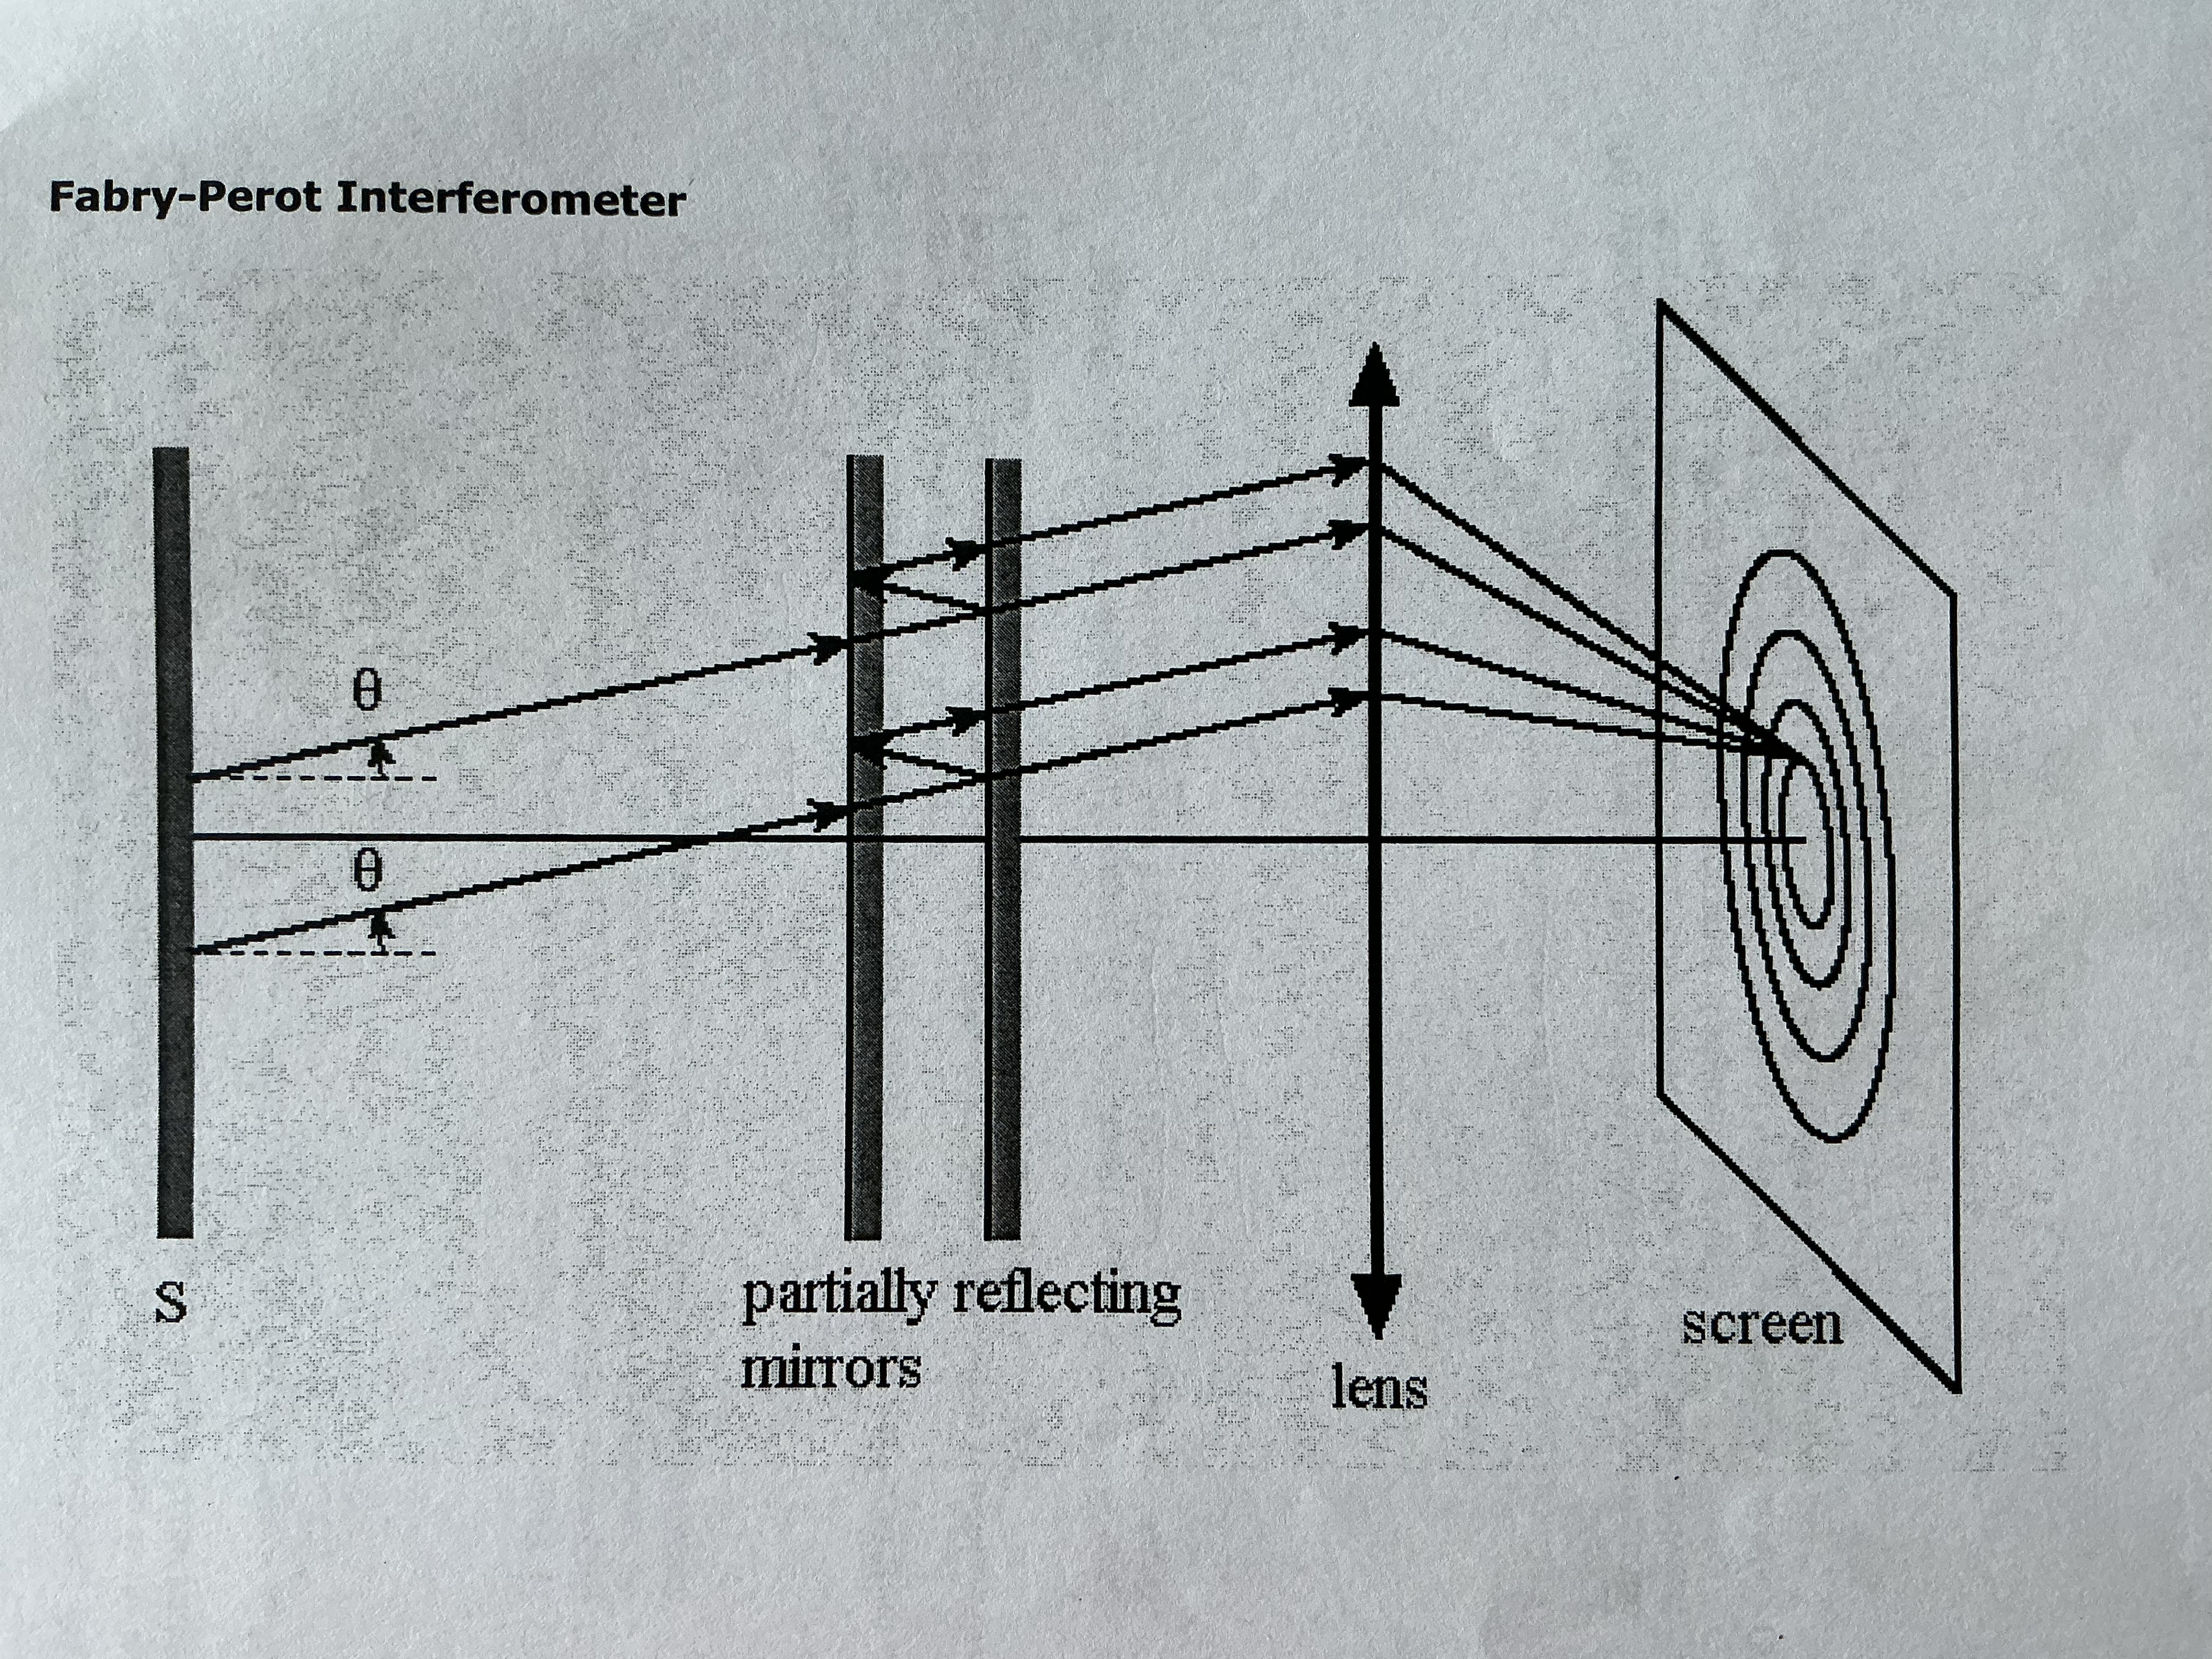
\includegraphics[width=0.35\textwidth]{Images/IMG_0228.png}

        \pagebreak
    \underline{Laser Beats}
        Laser on photodiode gives 2 peaks, which move up and down as filter is rotated;
        Polaroid creates beat
        \begin{gather*}
            f_B = \Delta f_L = \frac{c}{2L}
        \end{gather*}

    \underbar{Sodium Spectrum}

        Sodium light (usually yellow) split by magnet changes energy of electrons using magnetic field.
        \begin{gather*}
            E = \frac{hc}{\lambda} \to |\Delta E| = \frac{hc}{\lambda^2}|\Delta\lambda|\\
            d\sin(\theta) = m\lambda \to d\cos(\theta)\Delta\theta = m\Delta\lambda\\
            \lambda \approx 589.59\,\unit{\nano\meter}\\
            B = \frac{\Delta E}{2\mu_B} = \frac{n \mu_0 e \hbar}{2\pi m r^3}
        \end{gather*}
\end{document}